%%%%%%%%%%%%%%%%%%%%%%%%%%%%%%%%%%%%%%%%%%%%%%%%%%%%%%%%%%%%%%%%%%%%%%%%%%%%%%%%
\section{About Snakemake}
{   
	\usebackgroundtemplate{
		\vbox to \paperheight{\vfil\hbox to \paperwidth{\hfil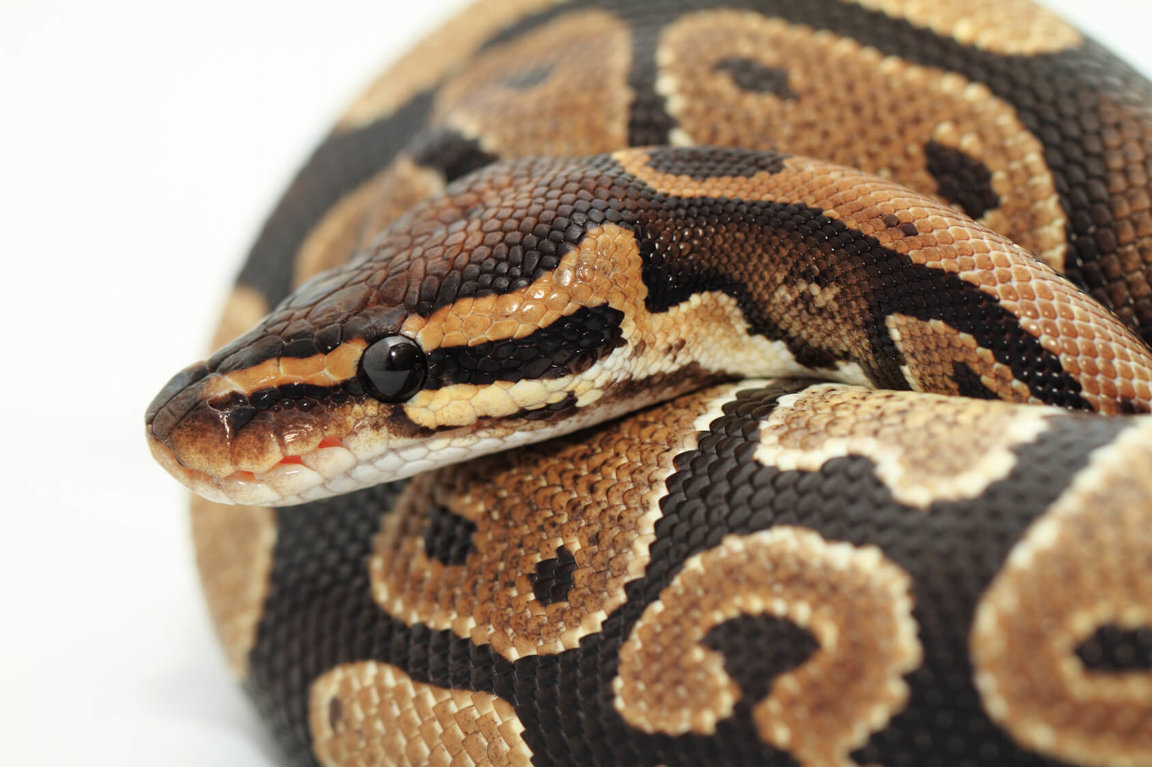
\includegraphics[height=\paperheight]{logos/Wild_Python.jpg}\hfil}\vfil}
	}
	\frame{
		\frametitle{Snakemake}
		\begin{mdframed}[tikzsetting={draw=white,fill=white,fill opacity=0.8,
				line width=0pt},backgroundcolor=none,leftmargin=0,
			rightmargin=150,innertopmargin=4pt,roundcorner=10pt]
			\tableofcontents[currentsection,sections={1-4},hideothersubsections]
		\end{mdframed}
	}
}

%%%%%%%%%%%%%%%%%%%%%%%%%%%%%%%%%%%%%%%%%%%%%%%%%%%%%%%%%%%%%%%%%%%%%%%%%%%%%%%%
\begin{frame}
	\frametitle{What is this about?}
	\begin{question}[Questions]
		\begin{itemize}
			\item Why \Snakemake?
			\item Why not "Something Else"?
			\item Why Clusters?
		\end{itemize}
	\end{question}
	\begin{docs}[Objectives]
		\begin{enumerate}
			\item Introduction to \Snakemake Usage (in-depth will follow)
			\item Get an Mini-Overview about Workflow Systems
		\end{enumerate}
	\end{docs}
\end{frame}

\subsection{\Snakemake and the Workflow Catalogue}

%%%%%%%%%%%%%%%%%%%%%%%%%%%%%%%%%%%%%%%%%%%%%%%%%%%%%%%%%%%%%%%%%%%%%%%%%%%%%%%%
\begin{frame}
	\frametitle{\Snakemake}
	\begin{figure}
		\centering
		\caption*{\textbf{>1e6} downloads since 2015\newline
			\textbf{>1300} citations\newline
			\textbf{>7} citations per week since 2021}
		
\includegraphics[width=0.6\textwidth]{Snakemake/paper_wall.png}
	\end{figure}
\end{frame}

%%%%%%%%%%%%%%%%%%%%%%%%%%%%%%%%%%%%%%%%%%%%%%%%%%%%%%%%%%%%%%%%%%%%%%%%%%%%%%%%
\begin{frame}
	\frametitle{The \Snakemake{} Catalogue}
	\begin{columns}
		\begin{column}{0.5\textwidth}
			\begin{itemize}[<+->]
				\item Extremely feature rich: \lhref{https://snakemake.github.io/snakemake-workflow-catalog/}{over 1800 workflows}
				\item Almost a hundred standardized workflows ready to use (meaning: well documented and with automatic deployment)
				\item Cluster batch systems are supported (and support for various cloud systems, too)
				\item There is an option to include Nextflow wrappers, too.
			\end{itemize}
		\end{column}
		\begin{column}{0.5\textwidth}
			\begin{figure}
				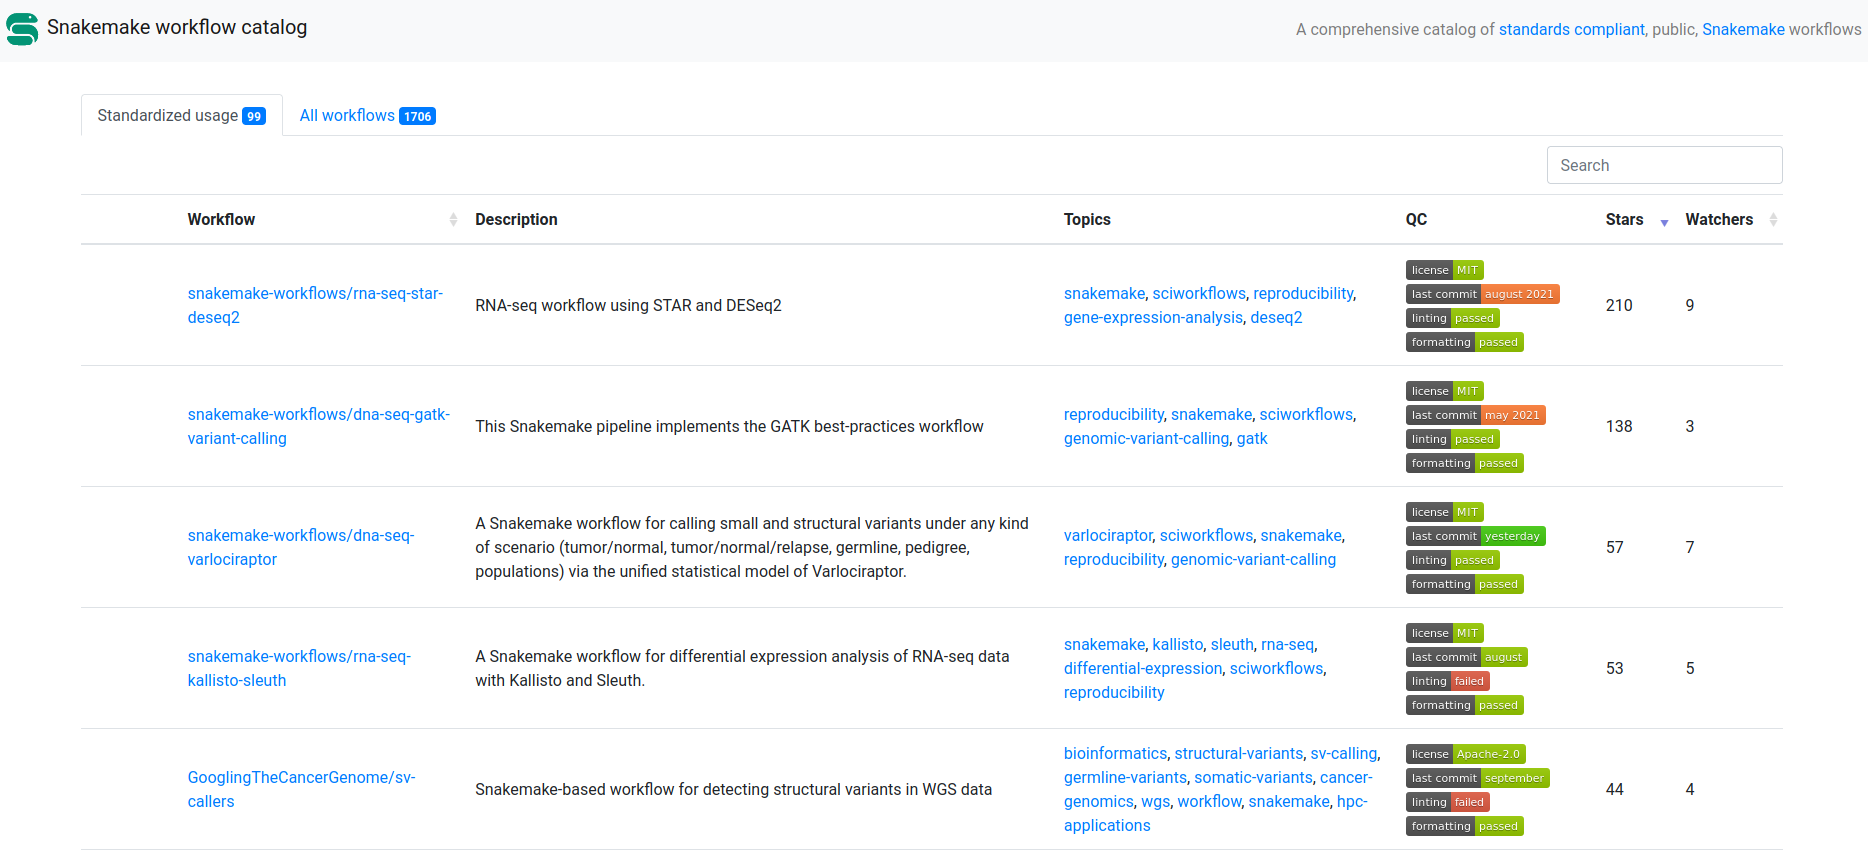
\includegraphics[width=\textwidth]{Snakemake/Snakemake_Workflow_Catalog.png}
				\caption*{Screenshot of the Workflow Catalogue}
			\end{figure}
		\end{column}
	\end{columns}
\end{frame}

%%%%%%%%%%%%%%%%%%%%%%%%%%%%%%%%%%%%%%%%%%%%%%%%%%%%%%%%%%%%%%%%%%%%%%%%%%%%%%%%
\subsection{Background}

%%%%%%%%%%%%%%%%%%%%%%%%%%%%%%%%%%%%%%%%%%%%%%%%%%%%%%%%%%%%%%%%%%%%%%%%%%%%%%%%
\begin{frame}[fragile]
	\frametitle{How does \Snakemake on a Cluster work?}
	\begin{columns}[T]
		\begin{column}{.5\textwidth}
			\begin{itemize}[<+->]
				\item Snakemake is triggered on the command line:
				\begin{lstlisting}[language=Bash, style=Shell]
$ snakemake [<arguments>]
				\end{lstlisting} 
			    \item you will fill in the parameters of your workflow (in a file)
			    \item Snakemake will run on the login-node and spawn your jobs on the cluster 
			\end{itemize}
			
		\end{column}
		\begin{column}{.5\textwidth}
			\only<3>{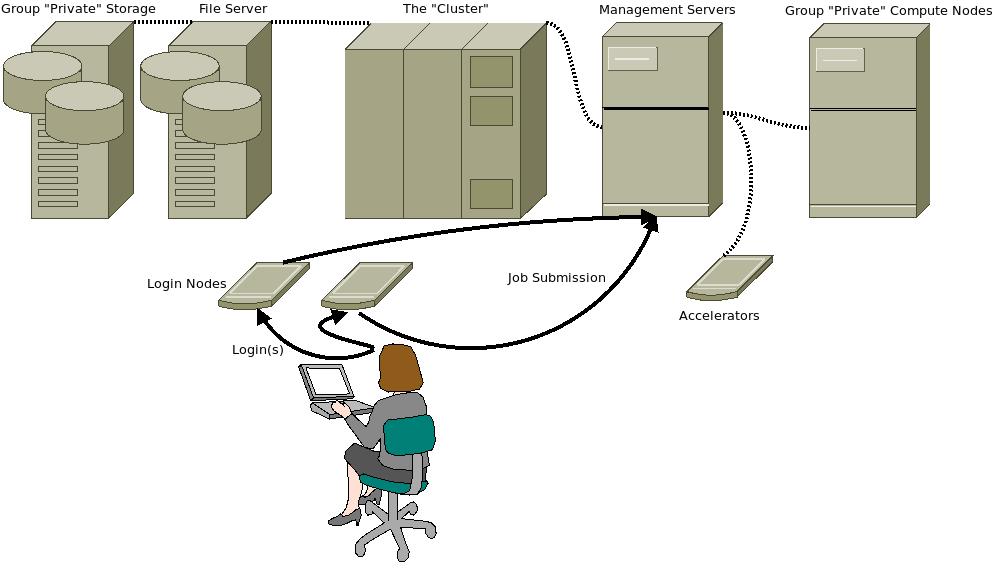
\includegraphics[width=0.95\textwidth]{misc/cluster_scheme.png}}
		\end{column}
	\end{columns}
\end{frame}

%%%%%%%%%%%%%%%%%%%%%%%%%%%%%%%%%%%%%%%%%%%%%%%%%%%%%%%%%%%%%%%%%%%%%%%%%%%%%%%%
\begin{frame}<handout:0>
  \frametitle{"Spawn Jobs on a Cluster?!" - What does it mean?}
  \centering
  \begin{tabular}{m{0.1\textwidth} m{0.25\textwidth} m{0.2\textwidth} m{0.45\textwidth}}
PC: & 
\includegraphics[width=0.1\textwidth]{misc/pc_color.png}  	    &  
\includegraphics[width=0.2\textwidth]{misc/sequential_code.png} &  \begin{minipage}{0.45\textwidth}
	$\Rightarrow$ sequential code \newline
	(perhaps parallel)
\end{minipage} \\ \pause
 	
Server: & 
\includegraphics[width=0.15\textwidth]{misc/homeserver.png}  	&  
\includegraphics[width=0.2\textwidth]{misc/concurrent.pdf} & \begin{minipage}{0.45\textwidth}
	$\Rightarrow$ sequential code \newline(perhaps parallel), \newline some concurrency
	\end{minipage}\\ \pause
  	
Cluster: & 
\includegraphics[width=0.15\textwidth]{misc/data_center.png}  	&  
\includegraphics[width=0.2\textwidth]{misc/high_concurrent.pdf} & \begin{minipage}{0.45\textwidth}
	$\Rightarrow$ programs launched \newline with high parallelism, \newline high concurreny
	\end{minipage}\\
  \end{tabular}
\end{frame}

%%%%%%%%%%%%%%%%%%%%%%%%%%%%%%%%%%%%%%%%%%%%%%%%%%%%%%%%%%%%%%%%%%%%%%%%%%%%%%%%
\begin{frame}
   \frametitle{Benefit of Cluster Usage}
   \begin{columns}
   	 \begin{column}{0.6\textwidth}
   	 	\centering
   	 	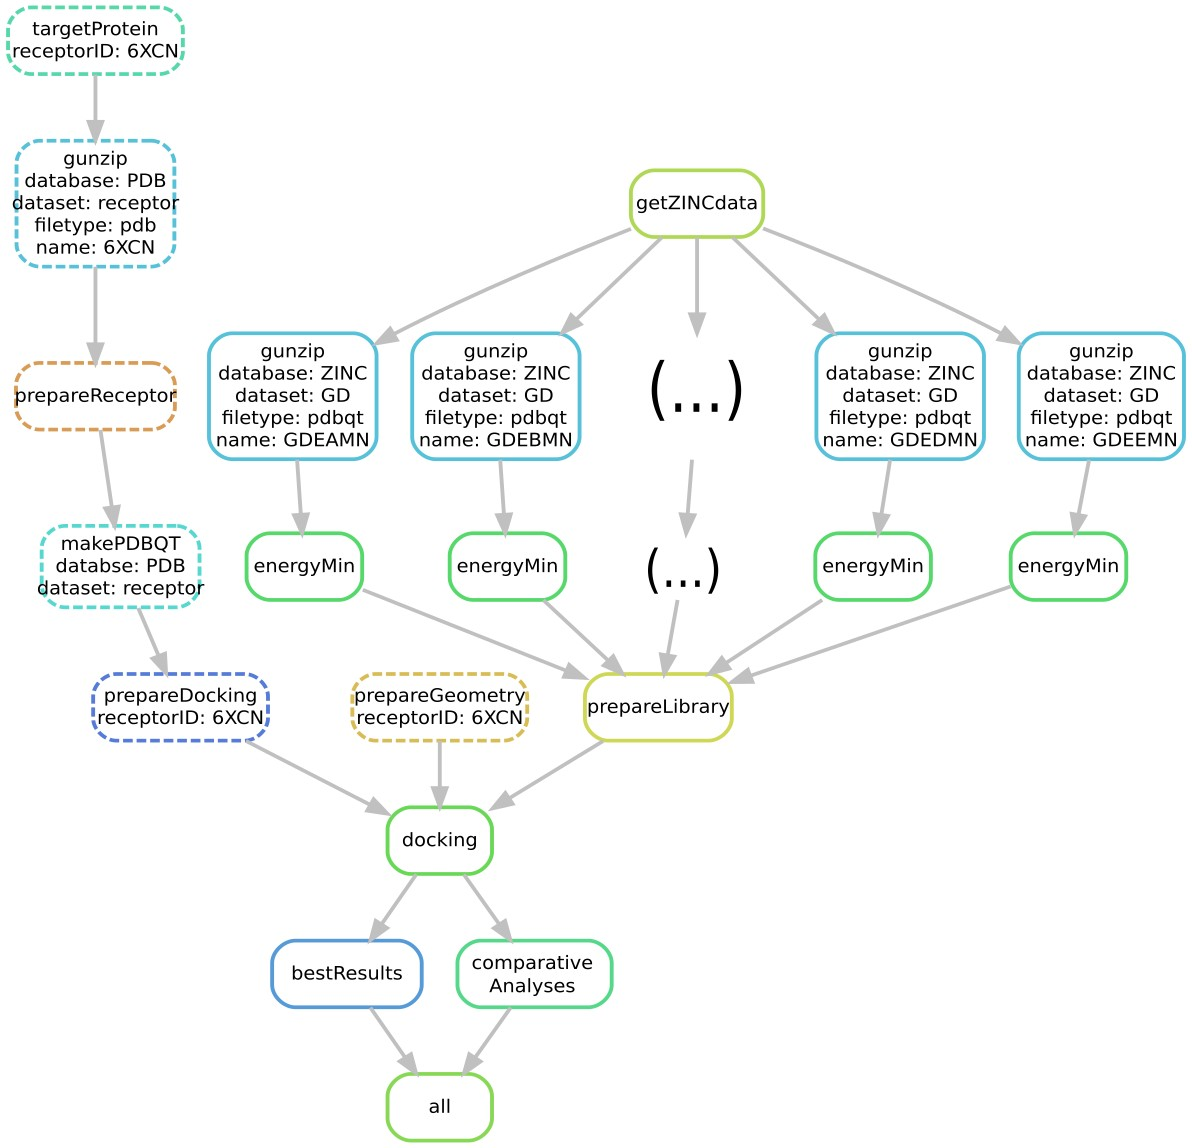
\includegraphics[width=0.8\textwidth]{workflows/molecular_screening_dag.jpeg}
   	 \end{column}
     \begin{column}{0.6\textwidth}
     	{\footnotesize
     		\Snakemake offers
     		\begin{itemize}[<+->]
     		  \item to carry out Nextflow wrappers
     		  \item to react on your input \newline $\Rightarrow$  more samples, more jobs
     		  \item to be a remedy to I/O contention
     		  \item to be ready for real time \newline computation with cluster support
     		  \item to support you from your input \newline to publication
     		  \item \ldots
     		\end{itemize}
     	}
     \end{column}
   \end{columns}
\end{frame}
	